% Chapter 2

\chapter{Literature Review} % Main chapter title

\label{Chapter2} % For referencing the chapter elsewhere, use \ref{Chapter1} 


\section{Introduction}
This research study aims to develop a framework of qualities or principles needed for a digital game to be used effectively within an educational environment as well as whenever a game attempts to impart information in general. As such, this research study applies to any educational game and “serious games”. This chapter will focus on available literature on several fields in an attempt to both explain the necessary background information and also perform a pseudo-meta-analysis on the available literature by presenting and then discussing what has already been done and what could still be done in each respective field, if applicable. These fields will include pedagogy, ludology and gamification as these are closely linked to the research question of this study. Pedagogy to discuss approaches to teaching, ludology to discuss the development and implementations of games and gamification to attempt to link the two.

\section{An Issue with Instructional Education}
Education, as it stands, is still built on a paradigm that is no longer needed in modern society. One major flaw with the current system is that it stifles the creativity and drive of some students as each level of education is largely the same and is, as such, monotonous (\cite{Ackoff2008}). Therefore, education requires some form of system to create an interest in learning for the students.
\\\\
Ackoff and Greenberg (2008) explain that the current traditional means of teaching are no longer as relevant as they once were as it is aimed to produce members of society that were likely to not question any fundamental aspects of how things operated. It is largely a system that focuses on teaching while disregarding learning as the last major stride in development in education was to industrialise it – having them operate efficiently like factories (\cite{Ackoff2008}). It is a system that is designed to keep moving often employing a “No Child Left Behind” policy which results in almost no time for anything other than the standardised and constantly measured curriculum (\cite{gibson2006games}). 


\begin{table}[H]
\centering
\caption{Organisational Needs Between the Industrial and Information Ages - Adapted from \cite{Reigeluth1996}}
\begin{tabular}{@{}l|l@{}}
\toprule
\textbf{Industrial Age} & \textbf{Information Age} \\ \midrule
Standardisation         & Customisation            \\
Adversarial relations   & Cooperative relations    \\
Compliance              & Initiative               \\
Conformity              & Diversity                \\
CEO as “king”           & Customer as “King”       \\ \bottomrule
\end{tabular}
\label{tab1}
\end{table}

This current paradigm of education is operated on the basis of standardisation to accommodate the change in societal needs and requirements that the industrial age brought with it (\cite{Reigeluth1996}). Reigeluth (1996) states that this system was developed on the fundamental need of sorting students into different categories and to allow for comparisons so that the training of the workforce could also be separated into different groups, those being labourers, having “hands-on” skills, and managers, who mainly had a managerial skill set. 
\\\\
However, with the shift into the “information age”, the requirements of the workforce have also changed. The industrial age being a time of mass-production with the emergence of various new processing technologies and the information age being characterised by the fact that information is being transmitted and generated at an ever-increasing rate due to further technological developments (\cite{gibson2006games, Reigeluth1996}). The most notable changes from the aforementioned paradigm shifts are that from conformity and compliance to initiative and diversity where greater value is placed on each individual’s strength and contribution to a project or organisation rather than each individual having the same skill set (\cite{Reigeluth1996}).  A few other differences between the needs of organisations during the industrial age and the new requirements brought with the information age are depicted in the above table.
\\\\
Reigeluth (1996) continues and states that the current paradigm is not focused on learning but rather categorisation. Ackoff (1991) hold a similar viewpoint stating that there is more of a focus on teaching rather than learning. It should be noted that teaching and learning are very distinct from one another as both can take place without the other (\cite{Ackoff1991}). Learning is defined as increasing one’s ability to perform an act effectively while trying to meet an objective through acquiring new knowledge whereas teaching is the process of providing this knowledge (\cite{Ackoff1991}). Through this, it is clear that institutions under this paradigm aim to give learners a verbose vocabulary to speak on topics that they do not fully comprehend (\cite{Ackoff1991}). 
\\\\
Due to this aforementioned paradigm shift and in what requirements are desired by most organisations in the information age, a shift in instructional theory is also needed – one such as going from making use of passive learning through traditional teaching means to one that is centred on active learning (\cite{Reigeluth1996}). These changes are discussed in more detail in the following section on pedagogy and learning theories and the means to accomplish them in the further sections on ludology and gamification.

\section{Pedagogy and Learning Theories}
As one of the outcomes of this research study is a framework that details qualities and principles for a digital game to effectively present knowledge and information to a user, one of the first areas to look towards and discuss is pedagogy which entails a general discussion about several learning and instructional theories as well as how motivation plays a role in learning. Pedagogy is the study of the transferal of knowledge in an educational environment through several lenses such as social, political and cultural (\cite{Li2012}). As such it encompasses the fields and discussions of instructional design and theory as well as any learning theories.

\subsection{Learner's at the Core of Learning}
Some instructional theories focus on students learning with minimal interaction with a teacher or instructor. Reigeluth (1996) refers to the learning methods that follow his ideology as ones where an instructor acts as an indirect guide to a class of learners instead of the typical “sage on the stage” structure of a lecture or presentation. 
\\\\
Two of these aforementioned theories are learning by doing and learning by teaching methods. Learning by doing functions on the principle that skills can be improved through practice and self-perfection on a particular topic or knowledge base (\cite{Fisch2009}). This means of instruction has become increasingly popular amongst companies where they are able to make use of “on the job” training as it allows for a person to be productive immediately as well as become more proficient at tasks gradually (\cite{Fisch2009}). The learning by teaching method works under the assumption that learners are able to increase their understanding of a certain topic by teaching it to other learners (\cite{Fisch2009}). This method of learning has garnered more usage recently as it is a viable means of learning in environments with too few teachers or instructors and increases the overall learning process (\cite{Fisch2009}). As shown in the following table, learning methods that place the learner in control are very flexible and as such can be incorporated when attempting to teach various and different fields or subjects (\cite{Ackoff1991}).

\begin{table}[H]
\caption{List of Several Learning Methods and Their Strengths - Adapted from (Moleda, 1995, as cited in \cite{Reigeluth1996})}
\begin{tabular}{@{}l|l@{}}
\toprule
Learning Method                          & Strengths                                                            \\ \midrule
Lectures or Presentations                & Efficient, Standardised and   Structured                             \\
Learners in Control                      & Very Flexible                                                        \\
Games and Simulations with a Rule System & \multirow{2}{*}{Increased Learner motivation and Knowledge Transfer} \\
Discovery as Individuals and Groups      &                                                                      \\ \bottomrule
\end{tabular}
\end{table}

As shown in the above table, using games and simulations as a means of learning is nothing new and it has been found that they have been used as instructional tools as far back as 3000 B.C in China (\cite{Dempsey1996}). Games are also a viable means of learning in a new paradigm of instructional design as it has been found to increase motivation amongst learners when used (\cite{Reigeluth1996}). The distinction between a game and a simulation is discussed in one of the following sections. However, the increased motivation this means of instruction brings is important and should be noted as providing learners, in all levels of education, with content through methods of delivery that they enjoy will, as previously stated, cause them to be more motivated to learn and thus look further into that specific topic themselves which circles back to the increased transfer of knowledge through discovery as an individual (\cite{Ackoff2008, Reigeluth1996}).

\subsection{Merrill's First Principles of Instruction}
Gibson et al. (2006) list and summarise several learning and instructional design theories that have the potential to be applied to a game used for learning. This study will, however, only look at 	Merrill’s First Principles of Instruction as it is the most recent of the ones depicted (\cite{gibson2006games}).
\\\\
Before discussing the principles that the name refers to in this theory, Merrill (2002) provides a few definitions for terms made use of. A principle in this context is a relationship that is always true regardless of the environment it is applied within (\cite{Merrill2002}). A practice is any instructional activity (\cite{Merrill2002}). A program is a means of instruction that makes use of several practices (\cite{Merrill2002}). Merrill (2002) states that the first principles described are able to be implemented in any instructional system or environment as they are “design-oriented” and as such relate more to creating learning environments rather than describing the means of knowledge transfer. Each of the following principles is also accompanied by three “corollaries” each of which Merrill (2002) likewise explains.
\\\\
The first principle of Merrill’s (2002) First Principles of Instruction is that the learning is problem centred. This principle describes three corollaries, the first of which being “Show Task” which states that learners should be shown the types of problems they will be solving or will be able to solve with the knowledge that they attain (\cite{Merrill2002}). The next is the “Task Level” which explains that the problems presented should keep learners engaged due to the complexity and not just the action of solving it (\cite{Merrill2002}). The last corollary, “problem progression” describes that the problems presented should have some form of increasing complexity while still being comparable to the previous iteration of the type of problem (\cite{Merrill2002}).
\\\\
The second principle is Activation which means that learning happens whenever previous experiences are used (\cite{Merrill2002}). The first corollary, “Previous Experience”, states that the learning process is enhanced when a learner is able to draw upon relevant past experiences and apply the associate knowledge as a foundation for new knowledge (\cite{Merrill2002}). “New Knowledge” is the second and explains that learners should be provided with a relevant experience as an additional foundation to add to their knowledge base (\cite{Merrill2002}). The last corollary is “Structure” and details that learners should be encouraged to organise new knowledge according to some relevant structure (\cite{Merrill2002}).
\newpage
The third principle, Demonstration, proposes that learning takes place when the activities that are undertaken impart the knowledge instead of stating the information (\cite{Merrill2002}). “Demonstration consistency” explains that any examples or visualisation should be kept in line with the original learning goals (\cite{Merrill2002}). The next is “Learner Guidance” and states that learners should be shown where the relevant information for problems can be found be it in the form of comparative examples or various representation of one source (\cite{Merrill2002}). “Relevant Media” explains that when media is used as a means of demonstration, different types can be used provided that they do not fight for a learner’s attention (\cite{Merrill2002}).
\\\\
The fourth principle is Application which states that learning takes place when learners actively solve problems with the new knowledge they have acquired (\cite{Merrill2002}). “Practice Consistency” is similar to Demonstration consistency but with a focus on the application of knowledge (\cite{Merrill2002}). “Diminishing Coaching” is where the learners are provided with relevant feedback, but it is slowly lessened over time (\cite{Merrill2002}). It is also important that the problems provided to learners for practice have a good variety, as explained as “Varied Problems” (\cite{Merrill2002}).
\\\\
The fifth, and final, principle is Integration which is when the knowledge a learner has acquired is used by them in their everyday life (\cite{Merrill2002}). The first corollary, “Watch Me”, explains that learners are provided to showcase the new knowledge or skill they have acquired (\cite{Merrill2002}). “Reflection” deals with giving learners time to be able to debate with others on the topic involved (\cite{Merrill2002}). Lastly, “Creation” states that learners should be able to make use of their new knowledge or skill in some personal capacity (\cite{Merrill2002}).


\begin{figure}[H]
\centering
\centerline{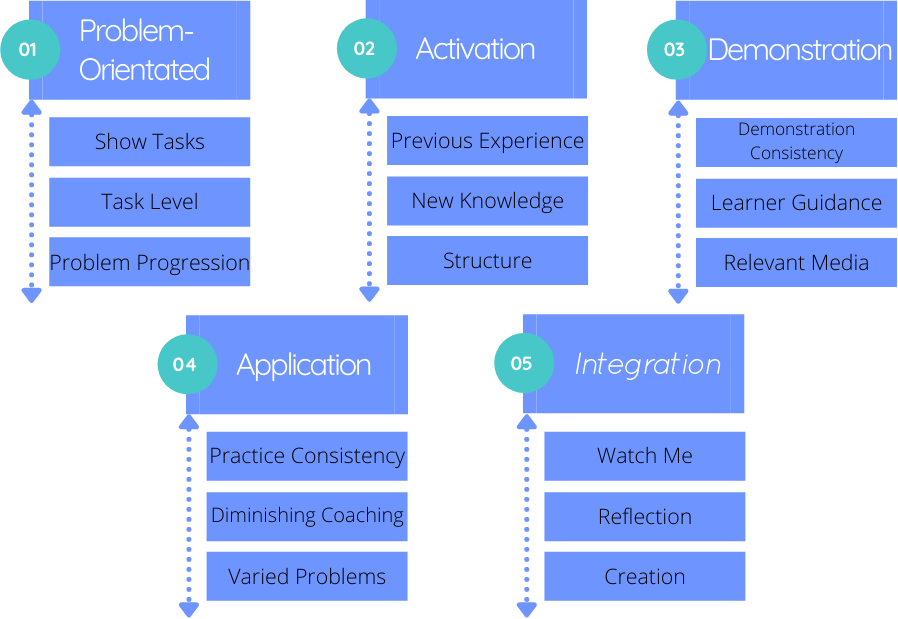
\includegraphics[scale=0.5]{Figures/merrill2.png}}
\caption{Own Image summarising Merrill's First Principles}
\end{figure}

The principles and corollaries provided by Merrill (2002) provide an expansive and detailed structure to be used when developing any learning opportunity making it an exceptional choice to adapt specifically to a digital game learning system.  It does, however, lack a comprehensive discussion on how to keep learners engaged with the content and, as such, the next subsection will discuss some theories pertaining to the role of motivation in learning.
\newpage
\subsection{The Influence of Motivation}
A learner's motivation is what will drive them to engage with and enjoy the content being studied. This motivation can come in one of two forms according to Kapp (2012a) and to better understand the theories focussed on learner motivation, this distinction will be discussed first.
\\\\
The first is intrinsic motivation which is any motivation aimed to accomplish something and has originated from a desire to do something for oneself (\cite{Kapp2012a}). Thus, the motivation comes from the learner. On the other hand, with extrinsic motivation, the drive and desire to accomplish a task of some kind stems from wanting some form of reward or avoiding punishment of some kind (\cite{Kapp2012a}). Thus, motivation is created in return for something, either tangible or otherwise. 
\\\\
One model for motivating learners is the ARCS Model which was developed by John Keller (1987) which is frequently referenced in the aforementioned field of instructional design (\cite{Kapp2012a}). It is comprised of four main elements with each focusing on designing instruction in a different way ((\cite{Kapp2012a, keller1987development})). 
\\\\
The first of these is Attention and it is an element that is concerned with gaining and then keeping the learners’ interest. There are three main methods to accomplish this with the first being gaining attention through the use of relatable examples or surprise. The next is to create curiosity within the learners through means such as role-playing or hands-on examples. The last means to keep attention is the variability which means periodically changing the method of delivery (\cite{Kapp2012a, keller1987development}).
\\\\
Relevance refers to having the content be relevant to the learner and Kapp (Kapp2012a) mentions that this can be done through orienting the environment around achieving goals, creating a link between the motives of learners and that of the instruction means, displaying that the content is in somewhat familiar to the learners and finally developing a model of the results of learning the presented knowledge (\cite{keller1987development}).
\\\\
Another element of this model, Confidence, is the expectations of success set by the learner and as such when they meet these expectations they are confident in their ability to do the work (\cite{Kapp2012a, keller1987development}). This can be aided by providing learners with clear expectations and requirements upfront about the skill or knowledge. It is also helpful to provide smaller opportunities to succeed as with each success the learners will become more confident (\cite{Kapp2012a, keller1987development}).
\\\\
The last element in the ARCS model is Satisfaction and is concerned with giving learners a sense of accomplishment and that the effort in the learning process has some value and weight to it (\cite{Kapp2012a, keller1987development}). This can be accomplished by allowing learners to see how their new-found knowledge can be used, either through the use of a real-world demonstration or via some form of simulation (\cite{Kapp2012a, keller1987development}).
\\\\
This section has detailed three aspects found within pedagogy, instructional design and learning theories each providing some insight into effectively transferring and imparting knowledge to a learner. Placing the learner at the centre of both teaching and learning allows for great flexibility in how to present that given material while Merrill (2002) provides an expansive framework to structure this presentation of knowledge whereas Kapp (2012a), through citing John Keller, explains ways to keep learners motivated throughout the learning process.

\newpage
\section{An Approach Through Ludology}
Another approach that could be taken is one that is rooted in games as these are popular among those in schools and as such should provide a means to deliver content in an interesting and engaging manner (\cite{Virvou2005}).
\\\\
To be able to implement a digital game as a means of learning, an understanding of games, in general, is needed. This section details ludology in general and the various applications and topics it encompasses ha relate in some manner to the research problem discussed. These topics will include a discussion on games as a means of simulation and what is referred to as a “serious game” within the field. 

\subsection{What is Ludology}
Ludology is the formal and academic study of games and has roots in studying games through a cultural and social lens by discussing how each interacts with the so-called “spirit of play” (\cite{Huizinga1949}). However, relatively recently, as early as 2001, the field has shifted and now encompasses the study of digital computer-based games as this is when the first academic peer reived journal on the topic was published as well as several international conferences taking place (\cite{Frasca2013}). 
\\\\
As such, this study will use the definition provided by Gonzalo Frasca, “Ludology can be defined as a discipline that studies games in general, and video games in particular” (\cite{Frasca2013}). Frasca (2013) further elaborates on his statement that the field of ludology has a focus on discussing and understanding the individual elements of games as well as creating models to explain the various mechanics and rules of games. 
\\\\
In its infancy, the field of ludology was heavily compared to narratology, the study of narratives as they were seen as nothing more than a new medium to demonstrate and display story-telling (Murray, 1997, as cited in \cite{Frasca2002}). Due to this digital and video games were studied under the same framework that would regularly be applied to drama, films and narratives as they unarguably had narrative elements in them to varying degrees (\cite{Manovich2002}). Frasca (2002) cites Espen Aarseth stating that studying digital games under a narratology framework was a misguided attempt at understanding them and digital games would require their framework to be studied under. Eskelinen (2001) echoes this mentioning that when games were studied, the discussions were centred within literary and film studies as games were depicted as interactive narratives. This definition of games has little substance to it and comes from a limited knowledge of, often outdated, literary theory (\cite{Eskelinen2001}).

\subsection{Serious Games}
Annetta (2008) states that the movement to include video games in teaching and training began in 2003, two years after the field of ludology began to gain traction itself concerning digital and computer-based games. The types of games used in this context are often referred to as “serious games”.  
\\\\
“Serious games” were introduced as digital concepts in 2002 through the Serious Game Initiative which was spearheaded by David Rejeski and Ben Sawyer (\cite{DeGloria2014}). The initial intention for serious games was for them to be used as a means of training certain tasks and skills (\cite{DeGloria2014}) – this was typically done through simulation type games which will be discussed in the following subsection in greater detail.
\\\\
Virvou, Katsionis and Manos (2005) mention that the endeavour to create serious games has yet to reach schools due to certain criticisms about games in general that hinders this. This is due to the fact that discussions around games by educators have largely focused on the social consequences of playing games instead of the educational potential games hold (\cite{Squire2003}). Due to this the study of serious games became more theoretical and discussion-based at lower levels and more applied with actual use at higher levels. This can be seen by implementations implemented in several fields including medical rehabilitation, ecological studies, learning languages and business studies (\cite{Burke2009, Costanza2014, Ranalli2008, Tao2009}). 
\newpage
These types of games have already had an impact on the military, medical and higher business education fields early in their conception and this trend continues to this day with most serious games being used within the medical fields specifically (\cite{Annetta2008, DeGloria2014}). However, there were attempts to use serious games, as simulations, within physics and engineering (\cite{Deshpande2011}).

\subsection{Games as Simulation}
Games have also found use as a means to simulate models, environments and a myriad of other systems. As mentioned in the previous subsection, there are a few games used for medical training (\cite{Burke2009}) and to be effective at teaching and demonstrating these topics, digital games need to be used as a simulation.
\\\\
Squire (2003) provides a definition for games as a simulation and states that these simulations attempt to model reality in a consistent manner usually through modelling physical or social systems through another system – which in this case would be a computer and the digital video game. There are two main types of simulations, Hi-fidelity and low fidelity. Hi-fidelity simulations attempt to model every possible interaction in a given system, phenomena or environment as accurately as possible (\cite{Squire2003}). In contrast, a low fidelity simulation will make use of a fair bit of abstraction as it aims to only demonstrate a few key characteristics of the phenomena or environment (\cite{Squire2003}). Games as simulations would comprise of both of these types depending on the content that it attempts to simulate,
\\\\
Deshpande and Huang (2011) describe the use of games as a means of simulation for specific sections of work in physics and engineering courses as an addition to traditional teaching as it provides a relatively simple way to demonstrate certain phenomena. As such these authors discuss the simulation aspect of games rather than the narrative as when dealing with a simulation digital game it typical lacks most narrative elements in the traditional sense (\cite{Deshpande2011}).
\\\\
This section detailed the field of ludology and its roots in the “spirit of play” amongst cultures and society as well as the shift into being an academic means to study digital computer games. Through this, it was able to describe and develop the idea of a “serious game” and consequently games as simulations which are the most effective means to convey a learning environment through video games as a whole. Following this section, this study discusses how to link the learning theories of the previous section and the study of games together through a specific discussion on gamification. 

\section{Gamification}
This section will discuss the process of gamification and the theoretical knowledge behind it. This field is crucial to what this research study wishes to accomplish as it is the link to transform traditional teaching and learning into a game-based structure. Furthermore, this section will focus on the aspects of gamification that can be applied and translated into a digital game. 
\\\\
Gamification can be defined as making use of game-like mechanics, aesthetics and thinking to create motivation, solve problems and produce a more suitable learning environment (\cite{Kapp2012a}). Kapp (2012b) states that while gamification makes use of game elements, it only makes use of a few of them as in a gamified system, in a gamification context, learners are not constantly engaged in playing the game as there are sections of respite from this, such as video explanations. While elements such as points and achievements are found in most games, gamification strives to add more than just these to a classroom as with the absence of other elements and only points and badges, the resulting system is one that is dull (\cite{KappArticle2012}). Kapp (2012b) continues stating that gamification adds much more to create an interesting system such as narrative aspects and continuous feedback to learners to create and upkeep their motivation and engagement with the system.
\newpage
Gamification is often not implemented within a classroom but is rather presented to learners through some external means – such as a digital game (\cite{KappArticle2012}). It should be noted, however, that a serious game can be the result of the gamification of some content but gamification does not always have to produce a serious game as a result (\cite{KappArticle2012}).  Kapp (2012a) describes various types of knowledge and how to begin developing a gamified system to effectively teach each of them:

\begin{itemize}
\item Declarative Knowledge is usually comprised of facts and jargon within a topic and is best taught by making use of sorting and matching type games.
\item Conceptual Knowledge is the grouping of related information that have an underlying common descriptor and is best taught by using demonstrations and sorting based on the common trait.
\item Rules-Based Knowledge is strict statements linking concepts and is best taught by demonstrating what failing to comply with the rules are.
\item Procedural Knowledge is a progression based path to reach an outcome and is best taught through the use of having learners work through the procedure in a demonstration and other means as well.
\item Soft Skills are general strategies for dealing with various social interactions and are best taught through the use of repeated application of the skill in different scenarios.
\item Affective Knowledge deals with topics about subjective phenomena such as emotions and is most effectively taught through immersing the learner within these phenomena.

\item Psychomotor Domain deals with making use of cognitive knowledge through physical skills (hand-eye coordination is an example of this) and is most effectively taught through observation.
\end{itemize}
Gamification makes use of several procedures and processes that are rooted in various academic theories, most notably ones found within pedagogy and as such was discussed in the pedagogy section of this literature review (\cite{KappArticle2012}).
\\\\
This section on gamification has thus discussed what gamification entails and how it usually implemented. A focus on the types of knowledge it is able to gamify is also presented as well as one way to effectively teach that type of knowledge. The following section will discuss existing attempts at producing a gamified system and serious games.
\newpage
\section{Existing Gamified Teaching Systems and Educational Games}
This section will detail various examples of previously implemented gamified teaching systems and educational games in an attempt to identify what approaches have already been detailed. Furthermore, this approach will also allow for the identification of which aspects are commonly used in educational systems and games among these implementations. 
\\\\
Dincelli and Chengalur-Smith (2020) developed a game with the intention to train employees on certain security issues such as social engineering through social media. This study developed two different gamified artefacts, one that made use of graphics and one that was entirely comprised of text, with both of them following a “choose your own adventure” approach where the narrative of the game shifts depending on the users’ choices or actions (\cite{Dincelli2020}).

\begin{figure}[H]
\centering
\centerline{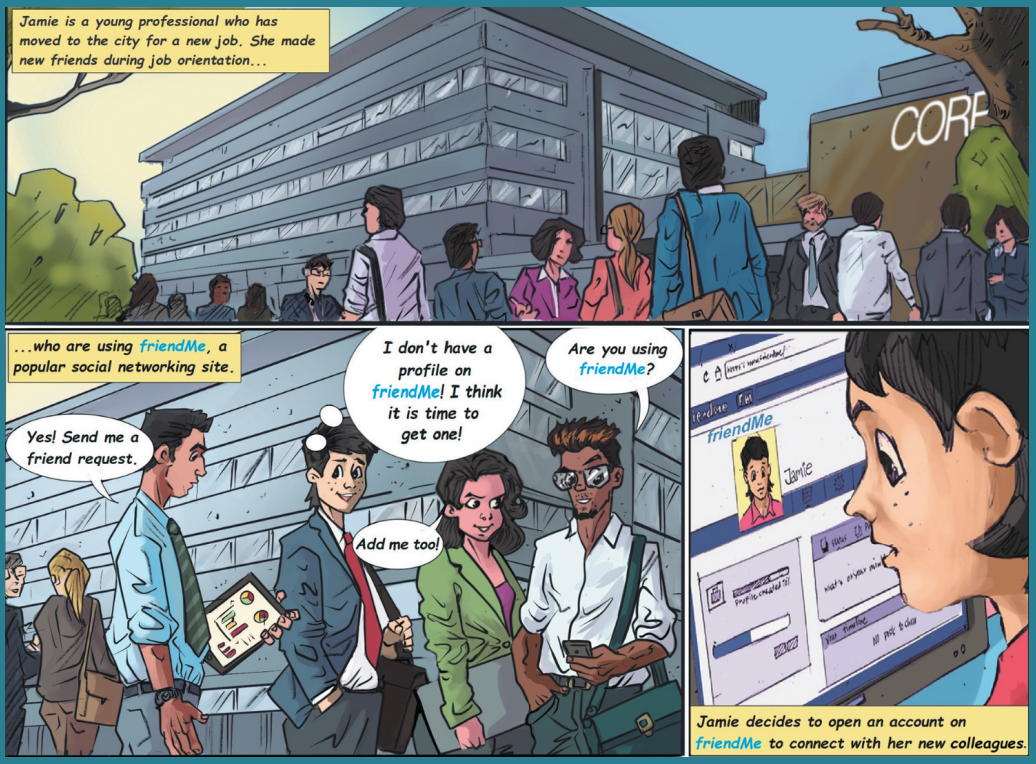
\includegraphics[scale=0.5]{seta.png}}
\caption{Example Frame from the SETA gamified training system – Reused from (\cite{Dincelli2020})}
\end{figure}

Dincelli and Chengalur-Smith (2020) discuss their approach to developing this artefact and make a few key decisions. The first is to apply some form of narrative, or story-based elements to the game, which allows for an agent to guide a user through the learning process presented (\cite{Dincelli2020, Sheng2007}). Another principle they made use of is reflection, which, when implemented, should provide time to users to think about the information and reflect on it (\cite{Dincelli2020, Sheng2007}). This study also goes on to mention further articles used in the construction of the artefact hen identifying what qualities they should make use of (\cite{Dincelli2020, Liu2017}). The conclusion this study came to was that a gamified system of any kind is more effective than traditional means and a game with graphics is easier for users to comprehend (\cite{Dincelli2020}).
\\\\
Annetta (2008) discusses multiple examples of educational games aimed towards younger audiences, such as Discover Babylon. This game was developed by the University of California in conjunction with several other institutes. It was a multiplayer game that made use of hi-fidelity simulation, as defined above, to accurately simulate mysteries around Babylon that are solved by garnering an understanding of the Mesopotamian society of the city (\cite{Annetta2008}). It was designed for children just entering their teen years and made use of 3D photorealistic renderings of the city, shown in the figure below, as well as a question and answer management system (\cite{Annetta2008}). 

\begin{figure}[H]
\centering
\begin{subfigure}{.5\textwidth}
  \centering
  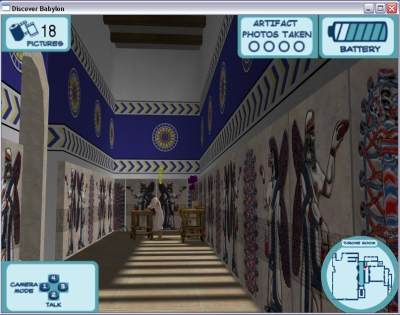
\includegraphics[width=0.84\linewidth]{Figures/baby.png}
  \caption{A Screenshot from Discover Babylon}
\end{subfigure}%
\begin{subfigure}{.5\textwidth}
  \centering
  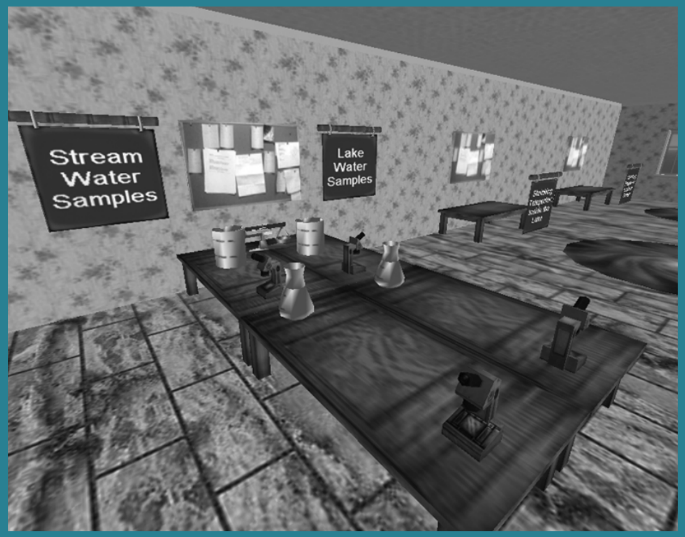
\includegraphics[width=0.84\linewidth]{Figures/wolf.png}
  \caption{A Wolf Den Minigame - Reused from (\cite{Annetta2008})}
\end{subfigure}
\caption{Examples of Serious Games used for Educational Purposes}
\end{figure}

The Wolf Den is a virtual learning environment developed at North Carolina State University as a means to facilitate online and distance learning (\cite{Annetta2008}). The system facilitated real-time communication between participants and allowed for students and teachers to engage in the development of role-playing games as well as a means to teach online courses (\cite{Annetta2008}). This system also allowed for various “minigames”, one such example being a digital laboratory designed to test water samples and interact with chemicals usually found within a chemistry lab – thus making use of hi-fidelity simulation as well (\cite{Annetta2008}).  The water testing lab example is pictured above;
\\\\
A brief look at three serious game examples has shown that for an educational institution learning game, hi-fidelity simulation is more often used as the topics discussed require a full array of interactions while serious games meant for employee training that does not directly teach skills pertinent to their job, low fidelity simulation with some form of narrative is a solid approach.

\section{Potential Effects of Game-Based Learning}
Lastly, this section will document various and effects of using game-based learning in an attempt to ensure the framework of qualities and principles developed can avoid introducing them into the system that will be developed. Specifically, this section will focus on several studies that discuss the effect of games or elements of games. 
\\\\
With the implementation of games as a means of learning, positive effects are wanted over others. A study had developed a digital game to illustrate the executive function of being able to switch attention from one task to another effectively and quickly and found that participants that had several hours of playtime performed better on cognitive tests that tested the aforementioned skill (\cite{Mayer2019}). This study also found that the increase in cognitive skills had not happened in some games but had in others, although they do not mention which games these are (\cite{Mayer2019}). 
\\\\
A study by Kristiadi et al. (2019) found that games that have an element of adventure to them tend to cause and develop positive behaviour in those who played them. This is, however, dependent on several other requirements as well such as representation based on knowledge morality, ethics and cooperation (\cite{Kristiadi2019}). 
\\\\
Mertala and Meriläinen (2019) conducted a study into what type of games children were most interested in and talked about in a meaningful way. The study found a few key influential games that most children mentioned, the most notable being Minecraft and Super Mario (\cite{Mertala2019}). The study goes on to discuss the “ideal game” that each child designed through a drawing and it is clear that, as with the aforementioned influential games, they are all vibrantly colourful (\cite{Mertala2019}).
\\\\
Wouters et al. (2013) conducted a meta-analysis into the motivational effects of serious games and as such discuss various motivation based theories. It was found that serious games are a more effective means of instruction than other contemporary methods (\cite{Wouters2013}). Wouters et al. (2013) also found that the motivation of the participants making use of the game was not statistically more significant than those using traditional methods. One reason for this may be found in an explanation of the self-determination theory of motivation, which links to intrinsic motivation defined above in this literature review (\cite{Wouters2013}).
\\\\
Gomez et al. (2019) conducted a study into what effects prolonged exposure to playing a popular game franchise, Pokémon, as a child would have later in life as an adult. The study made use of several images and took images of the brain’s activity in participants while showing them these different images, examples of these pictures are shown below in the figure (\cite{Gomez2019}). The study found that people who did play Pokémon extensively as children, had different activity in their visual cortex when looking at the image of a Pokémon as compared to the other images in addition to the other participants, those who had no interaction with Pokémon growing up, had almost no activity when looking at images of Pokémon (\cite{Gomez2019}). Gomez et al. (2019) suggest that during the period of early development that participants were exposed to Pokémon is also when the brain is most responsive to visual stimuli.

\begin{figure}[H]
\centering
\centerline{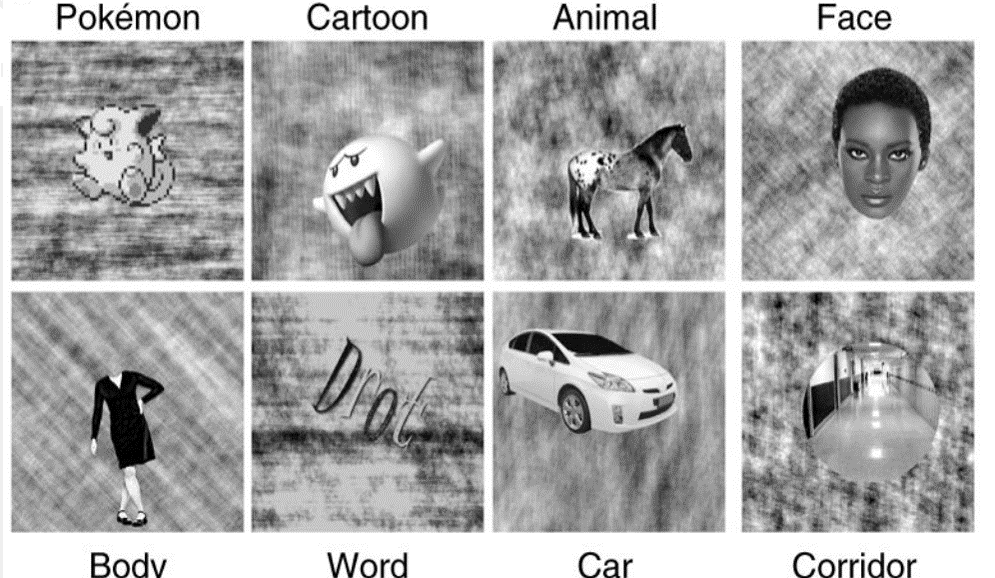
\includegraphics[scale=0.5]{Figures/poke.png}}
\caption{Example Images Used in The Study – Reused form (\cite{Gomez2019})}
\end{figure}


\section{Conclusion and Summary}
This chapter has discussed various fields of knowledge required to develop a framework of qualities needed by a serious or educational game to effectively teach a learner the content it deals with. The fields of pedagogy, ludology and gamification were discussed in addition to several case studies to further understand what is required. 
\\\\
When focusing on each of these fields with a lens focusing on developing this study’s framework, it is apparent that there is overlap between all three fields even without making use of gamification as a link between ludology and pedagogy. Gamification makes heavy reference to theories stated within the field of pedagogy as well as, as per its’ definition, borrows elements from ludology (\cite{KappArticle2012}). The most notable overlap between all three fields is that all make reference to narratology in some shape or form – pedagogy referring to including relatable examples, ludology being compared to narratology as a whole and gamification mentioning that involving stories is needed to teach certain knowledge types (\cite{Dincelli2020, Frasca2013, Kapp2012a, Sheng2007}). This was also shown in one of the case studies where story elements were used in a gamified training system (\cite{Dincelli2020, Sheng2007}). 
\\\\
Both gamification and pedagogy have means within their respective fields to gauge the effectiveness of teaching and learning through the use of some framework or principles (\cite{Kapp2012a, Merrill2002, Reigeluth1996}) while ludology only provides a framework to develop the games through the lens of game rules and mechanics (\cite{DeGloria2014}) and as such gamification provides a good base for developing a framework, much like Merrill’s in pedagogy, based within the field of ludology.


